% コンパイル: lualatex paper_ja.tex
\documentclass[10pt,twocolumn]{ltjsarticle}
\usepackage{luatexja-fontspec}
\usepackage[a4paper,margin=18mm]{geometry}
\usepackage{graphicx}
\usepackage{amsmath}
\usepackage{amssymb}
\usepackage{booktabs}
\usepackage{enumitem}
\usepackage[hidelinks]{hyperref}

\setlength{\columnsep}{6mm}

\begin{document}

\twocolumn[{%
  \begin{center}
    {\LARGE\bfseries 12Bパラメータ画像生成モデルへのキャラクタLoRA微調整}\\
    \vspace{0.6em}
    {\large ——消費者向け単一GPU上でのFP8量子化とブロックスワップ、および蒸留モデルへの転移——}\\
    \vspace{1.2em}
    {\large Masato Suzuki (Masafy)}\\
    \vspace{0.4em}
    {2026年6月25日}
  \end{center}
  \vspace{1.0em}
  {\centering\textbf{要 旨}\par}
  \vspace{0.4em}
  \begingroup\small
  \noindent 本報告では、著者の先行研究（Stable Diffusion~1.5 に対するキャラクタLoRA微調整）を、約12倍の規模を持つ最新の画像生成モデル \textbf{Krea~2}（Qwen-Image 系の単流 MMDiT、約120億パラメータ、フローマッチング）へと拡張する。先行研究と同一の被写体（著者が個人制作したレッサーパンダキャラクター「マサフィー」）と同一のハードウェア（VRAM 12\,GB の NVIDIA GeForce RTX~3060 単体）を用い、120億パラメータの拡散トランスフォーマに対する低ランク適応（LoRA）学習が消費者向け単一GPUで成立するかを検証した。鍵となる技術は、(i) 主要28ブロックへの動的スケール FP8 量子化、(ii) 最大26ブロックの CPU へのブロックスワップ、(iii) PyTorch のメモリ断片化対策（\texttt{expandable\_segments}）の三者併用であり、これにより VRAM ピークを 12\,GB 以内に収めた。学習は蒸留前の RAW モデルに対して行い、推論は8ステップ蒸留版 Turbo モデルで実行する転移構成を採った。13枚の参照画像から1{,}300ステップ（約8.4時間）の学習を行った結果、(a) 同一性を保持したキャラクタ生成が成立し、RAW で学習した LoRA が Turbo 推論へ良好に転移すること、(b) 学習エポック数の増加に伴い全体造形は強化される一方で、目のキャッチライト等の\emph{高周波の細部}が先に失われる過適合が観察されること、(c) この劣化は LoRA 適用強度の低減とプロンプト条件付けにより推論時に回復可能であること、を実験的に示した。本研究は、有料クラウド資源を用いずとも、120億パラメータ級の最新モデルに対する個人キャラクタの追加学習が消費者向けGPU 1台で実用的に完結することを示すものである。

  \par\medskip
  \noindent\textbf{キーワード:}\ 画像生成, 拡散トランスフォーマ, MMDiT, フローマッチング, 低ランク適応, LoRA, FP8量子化, ブロックスワップ, モデル蒸留, 消費者向けGPU
  \endgroup
  \vspace{2.0em}
}]

\section{はじめに}
著者は先行研究~\cite{suzuki2026sd15lora} において、個人制作のオリジナルキャラクター「マサフィー」（レッサーパンダを主題とし、メッセージングアプリ向けスタンプとして公開済み）を、潜在拡散モデル Stable Diffusion~1.5（SD~1.5; 雑音予測器の規模は約10億パラメータ）に対する低ランク適応（Low-Rank Adaptation; LoRA）で追加学習し、VRAM 12\,GB の消費者向けGPU 1台のみで実用的な生成が可能であることを示した。

その後の約1年間で、画像生成モデルのアーキテクチャは U-Net を基盤とする潜在拡散モデルから、\emph{拡散トランスフォーマ}（Diffusion Transformer; DiT）~\cite{peebles2023dit} および\emph{マルチモーダル拡散トランスフォーマ}（MMDiT）~\cite{esser2024sd3} を基盤とし、学習目的も DDPM 型の雑音予測から\emph{フローマッチング}~\cite{lipman2023flowmatching} へと移行した。本研究が対象とする Krea~2 はその代表例であり、Qwen-Image~\cite{qwenimage2025} 系の単流 MMDiT を骨格とし、約120億パラメータを有する。これは先行研究で用いた SD~1.5 の雑音予測器のおよそ12倍の規模である。

ここで自然な問いが生じる。\emph{先行研究で示した「消費者向け単一GPUでの個人キャラクタ学習」という枠組みは、規模が一桁増大した最新モデルに対しても依然として成立するのか。} 単純に考えれば、120億パラメータのモデルは半精度（bf16）でも約24\,GBを占め、12\,GBのGPUには重みすら載らない。したがって、何らかのメモリ圧縮・退避機構なしには学習は原理的に不可能である。本研究の中心的な貢献は、この制約を FP8 量子化とブロックスワップの併用により克服し、実際に学習を成立させた点にある。具体的な研究設問は以下の3点である。
\begin{itemize}[leftmargin=2.2em,topsep=2pt,itemsep=1pt]
  \item[\textbf{Q1.}] 半精度で重みのみ約24\,GBを要する120億パラメータの MMDiT に対し、VRAM 12\,GB の単一GPUで LoRA 学習を成立させられるか。成立させるための必要条件は何か。
  \item[\textbf{Q2.}] 蒸留前の RAW モデルで学習した LoRA は、少数ステップ蒸留版である Turbo モデルでの推論へ転移するか。
  \item[\textbf{Q3.}] 学習エポック数の増加は品質をどのように変化させるか。とりわけ細部（高周波成分）と全体造形（低周波成分）は同様に振る舞うか。
\end{itemize}
本論文の貢献は、これらに対する実験的回答を、再現可能な手順とともに提示する点にある。

\section{関連研究}
本研究は、拡散トランスフォーマ、フローマッチング、低ランク適応、被写体駆動生成、および学習の省メモリ化という研究系譜の交点に位置づけられる。

\textbf{拡散モデルと拡散トランスフォーマ。} 拡散確率モデルの実用的定式化は Ho ら~\cite{ho2020ddpm} の DDPM に始まり、Rombach ら~\cite{rombach2022ldm} の潜在拡散モデル（LDM）が高解像度合成の計算効率を改善した。その後 Peebles と Xie~\cite{peebles2023dit} は U-Net をトランスフォーマで置換した DiT を提案し、Esser ら~\cite{esser2024sd3} は画像とテキストのトークンを統合的に扱う MMDiT と整流フロー目的を導入した。Krea~2 が採る単流 MMDiT はこの系譜に連なる。

\textbf{フローマッチング。} Lipman ら~\cite{lipman2023flowmatching} は、雑音から データへの連続正規化流を回帰的に学習するフローマッチングを提案した。Krea~2 を含む近年の MMDiT 系モデルは、DDPM 型の雑音予測に代えてこの枠組みを採用する。本研究の損失（式\eqref{eq:fmloss}）はこの定式化に基づく。

\textbf{低ランク適応。} LoRA は Hu ら~\cite{hu2022lora} により大規模言語モデルの効率的微調整手法として提案され、その後 Transformer 一般、さらに拡散モデルへ応用が拡大した。本研究は LoRA を MMDiT の線形層へ適用する。

\textbf{被写体駆動生成。} 少数参照画像から特定被写体をモデルに束縛する課題は被写体駆動生成と呼ばれ、Ruiz ら~\cite{ruiz2023dreambooth} の DreamBooth が代表的である。本研究のトリガー語 $\tau$ による概念束縛はこの系譜に連なる。

\textbf{学習の省メモリ化。} 限られた VRAM で大規模モデルを扱うため、本研究では低精度数値表現と層単位の退避を併用する。FP8 は Micikevicius ら~\cite{micikevicius2022fp8} により深層学習向け数値形式として整理された。層を逐次 CPU と GPU の間で入れ替えるブロックスワップ（あるいはオフロード）は、近年の大規模生成モデルの学習器で広く実装される実務的手法である。本研究で用いた学習器 Musubi Tuner~\cite{musubi2026} はこれらを統合的に提供する。

\textbf{モデル蒸留。} 多ステップの拡散・フロー推論を少数ステップへ蒸留する手法は推論コストを大幅に削減する。Krea~2 の Turbo は RAW を8ステップへ蒸留した版であり、本研究は「RAW で学習し Turbo で推論する」転移構成を実証的に検討する。

\section{準備：理論的背景}
\subsection{フローマッチングと拡散トランスフォーマ}
データ $x_1\sim p_{\text{data}}$ と標準正規雑音 $x_0\sim\mathcal{N}(0,\mathbf I)$ を結ぶ時刻 $t\in[0,1]$ の補間を、最も単純な直線経路
\begin{equation}
x_t=(1-t)\,x_0 + t\,x_1
\label{eq:interp}
\end{equation}
で与える。対応する目標速度場は $v^\star=x_1-x_0$ である。ネットワーク $v_\theta$ は条件 $c$ のもとでこの速度場を回帰し、学習は条件付きフローマッチング損失
\begin{equation}
\mathcal{L}(\theta)=\mathbb{E}_{x_0,\,x_1,\,t}\Big[\,\big\lVert v_\theta(x_t,t,c)-(x_1-x_0)\big\rVert_2^2\,\Big]
\label{eq:fmloss}
\end{equation}
の最小化として行われる。推論では学習した速度場に沿って常微分方程式 $\mathrm{d}x_t/\mathrm{d}t=v_\theta(x_t,t,c)$ を $t:0\to1$ に積分する。Krea~2 では $v_\theta$ が単流 MMDiT で実現され、画像潜在トークンとテキスト条件トークンが共通の自己注意層を通じて相互作用する。条件 $c$ はテキストエンコーダ（Qwen3-VL-4B）の中間層特徴であり、画像オートエンコーダには Qwen-Image VAE を用いる。

\subsection{解像度依存の時刻シフト}
フロー系モデルでは、学習時の時刻 $t$ の分布を解像度に応じてシフトさせることが品質に寄与する。本研究では時刻を単調写像
\begin{equation}
t' = \frac{\sigma\, t}{1+(\sigma-1)\,t}
\label{eq:shift}
\end{equation}
で歪める\emph{シフト}を用いる。$\sigma$ はシフト係数であり、$1024\times1024$ では $\sigma=2.5$ が Krea~2 の推論時シフトに整合する（後述）。

\subsection{低ランク適応}
線形層の重み $W_0\in\mathbb{R}^{d_\text{out}\times d_\text{in}}$ を凍結し、低ランク差分 $\Delta W=BA$（$A\in\mathbb{R}^{r\times d_\text{in}},\,B\in\mathbb{R}^{d_\text{out}\times r}$, $r\ll\min(d_\text{in},d_\text{out})$）のみを学習する。順伝播は
\begin{equation}
h = W_0 x + \frac{\alpha}{r}\,B A x
\label{eq:lora}
\end{equation}
であり、$\alpha$ はスケーリング係数である。推論時には適用強度 $\lambda$ を導入して $h=W_0x+\lambda\,\frac{\alpha}{r}BAx$ とすることで、学習後に LoRA の効きを連続的に調整できる。本研究はこの $\lambda$ を品質制御の手段として活用する（第\ref{sec:results}節）。

\subsection{FP8量子化とブロックスワップによる省メモリ化}
\label{sec:mem}
120億パラメータのモデルは bf16 で約24\,GBを占め、12\,GBのGPUには載らない。本研究は次の三者を併用してこれを克服する。
\textbf{(i) FP8スケール量子化。} MMDiT の主要28ブロックの重みを読み込み時に動的スケール FP8（E4M3）へ量子化し、重みメモリをおよそ半減させる。正規化層を含む補助部はbf16に保つ。
\textbf{(ii) ブロックスワップ。} 主要ブロックのうち最大26ブロック（$=28-2$）を CPU 主記憶に常駐させ、計算の直前にのみ GPU へ転送する。これにより GPU に常駐する重みをさらに削減する。
\textbf{(iii) メモリ断片化対策。} PyTorch のキャッシュアロケータを \texttt{expandable\_segments} モードに切り替え、予約済みだが未割当の断片を再利用可能にする。
学習中はテキストエンコーダと VAE の出力を事前計算してディスクへ退避するため、学習ステップ本体では MMDiT のみが GPU を占有する。

\section{問題設定}
著者が制作したキャラクター「マサフィー」のスタンプ全16点から、品質基準により13点を選定して学習データ $\mathcal{D}=\{(x^{(i)},y^{(i)})\}_{i=1}^{13}$ とする。各 $y^{(i)}$ はトリガー語 $\tau=\texttt{masafee}$ を先頭に置いたタグ列のキャプションである。目標は、$\mathcal{D}$ から LoRA パラメータ $\phi=\{A_\ell,B_\ell\}_\ell$ を学習し、推論時に未収録のポーズ・場面を指定するテキスト $y$ に対して同一性を保持した画像を生成することである。先行研究との公平な比較のため、被写体・GPU・トリガー語・データ選定（13点）は先行研究と一致させ、相違点をアーキテクチャ（SD~1.5 $\to$ Krea~2）と学習基盤に限定する。

\section{手法}
\subsection{モデルとデータの準備}
拡散モデルには Krea~2 RAW（単一 \texttt{safetensors}、約24\,GB）を用いる。テキストエンコーダは Qwen3-VL-4B（bf16）、オートエンコーダは Qwen-Image VAE である。学習に先立ち、(1) VAE による画像潜在の事前キャッシュ、(2) テキストエンコーダ出力の事前キャッシュ、を行い、学習ステップ中のエンコーダ・VAEの常駐を回避する。学習画像は $1024\times1024$ にバケッティングする（原画像は $1000\times1000$）。

\subsection{学習設定}
LoRA は MMDiT の線形層に階数 $r=32$、$\alpha=32$ で挿入する。最適化は AdamW、学習率 $1\times10^{-4}$、バッチサイズ1、勾配チェックポインティング有効。時刻サンプリングはシフト（式\eqref{eq:shift}、$\sigma=2.5$）、損失は式\eqref{eq:fmloss}。総ステップ数は $13\times10=130$ ステップ/エポック $\times$ 10エポック $=1{,}300$ ステップ。VRAM制約への対応として第\ref{sec:mem}節の (i)--(iii) をすべて適用し、ブロックスワップ数は上限の26とした。2エポックごとに中間チェックポイントを保存する。

\subsection{推論設定と転移}
推論は8ステップ蒸留版 Turbo（メモリ節約のため GGUF~Q5\_K\_M 量子化）を用いる。RAW で学習した LoRA を Turbo の MMDiT に適用し、サンプラー \texttt{er\_sde}、スケジューラ \texttt{simple}、ステップ数8、ガイダンス強度 $s=1.0$（Turbo は CFG 不要）で生成する。これにより、学習は高精度な RAW で行いつつ、推論は高速・省メモリな Turbo で行う構成を実現する。

\section{実験}
学習および推論は、自宅に設置した単一の消費者向けGPU（NVIDIA GeForce RTX~3060、VRAM 12\,GB、ドライバ 595.71.05）を搭載した Linux PC（主記憶 30\,GB、PyTorch 2.6.0+cu124）上で完結させた。クラウドの有料計算資源は一切用いていない。学習中は GPU の消費電力・温度・VRAM占有・スループットを記録した。評価は次の三観点で行う。(E1) 学習の成立とリソース挙動、(E2) 同一性の獲得と RAW$\to$Turbo 転移、(E3) エポック数に対するアブレーションと推論時介入による品質制御。生成比較では、エポック間の差を明瞭にするため同一プロンプト・同一乱数種を用いる。

\section{結果}
\label{sec:results}
\subsection{E1：学習の成立とリソース挙動}
第\ref{sec:mem}節の三者併用により、120億パラメータの MMDiT に対する LoRA 学習が VRAM 12\,GB の単一GPUで\emph{成立した}。VRAM占有のピークは約11.9\,GB（容量の約97\%）であり、12\,GBにわずかな余裕を残して収まった。なお、断片化対策 \texttt{expandable\_segments} を適用しない条件では、学習ステップ2において約136\,MiBの追加割当に失敗して停止した（このとき約1.4\,GiBが予約済み未割当の断片として滞留していた）。すなわち、本規模では FP8 量子化とブロックスワップに加えて断片化対策が\emph{実効的な必要条件}であった。

学習スループットは約23.2\,秒/ステップであり、1{,}300ステップの総学習時間は8時間23分であった。図\ref{fig:loss} に学習損失の推移を示す。損失は学習初期に上昇したのち単調に減少し、終盤は約0.027前後で平坦化した。GPUは学習中ほぼ100\%稼働し、温度は69--75\,$^\circ$Cの安全域、消費電力は135\,W（電力上限170\,Wの約80\%）で推移した。これらは、消費者向けGPUが本規模の学習を熱・電力の面でも余裕をもって持続できることを示す。

\begin{figure}[t]\centering
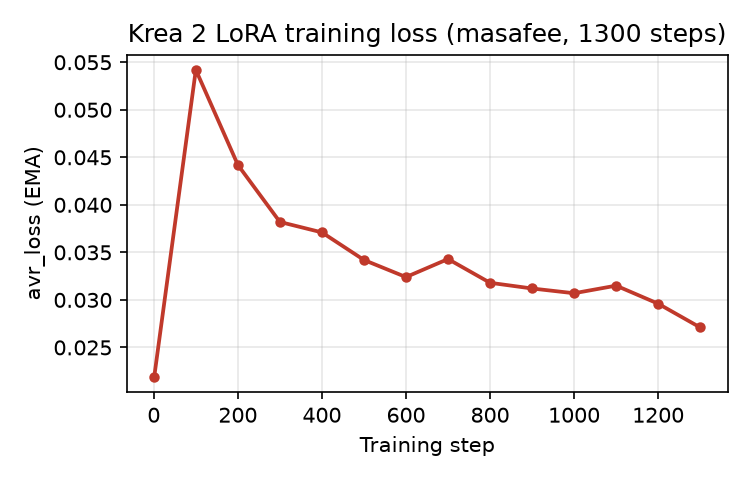
\includegraphics[width=0.96\columnwidth]{figures/fig_loss.png}
\caption{学習損失（指数移動平均）の推移。初期に上昇したのち単調減少し、終盤に約0.027で平坦化する。総1{,}300ステップ、約8.4時間。}
\label{fig:loss}
\end{figure}

\subsection{E2：同一性の獲得とRAW→Turbo転移}
図\ref{fig:identity} に、同一プロンプト・同一乱数種における LoRA 非適用（ベース Turbo）と LoRA 適用の比較を示す。ベースは汎用的なレッサーパンダを生成するのみであるのに対し、LoRA を適用すると、ゴーグル・王冠柄の衣装・縞模様の尾といったマサフィー固有の意匠が一貫して再現される。RAW で学習した LoRA がそのまま Turbo の8ステップ推論で機能していることから、\emph{RAW→Turbo の転移は良好に成立する}と結論づけられる。これは、学習を高精度モデルで行い推論を蒸留モデルで行うという分業が実用的に有効であることを示す。

\begin{figure}[t]\centering
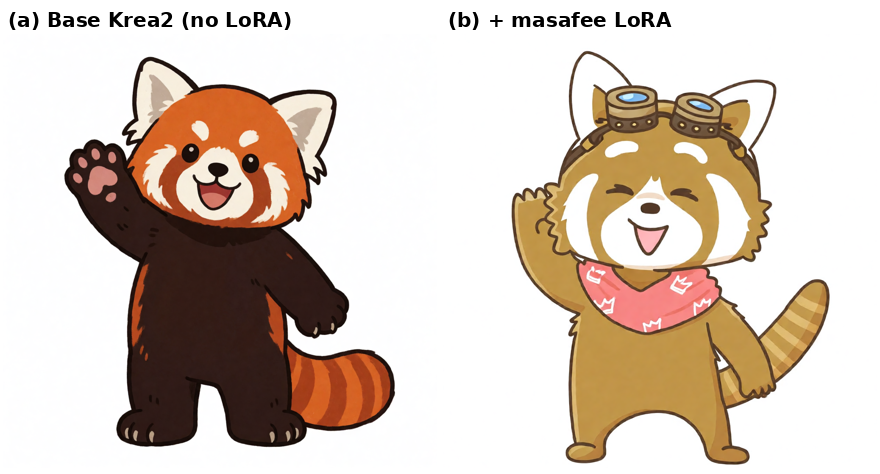
\includegraphics[width=0.96\columnwidth]{figures/fig_identity.png}
\caption{同一プロンプト・同一乱数種での比較。左：LoRA非適用（ベース）、右：LoRA適用。後者はゴーグル・王冠柄衣装・縞尾といった固有意匠を再現する。}
\label{fig:identity}
\end{figure}

\subsection{E3：エポックアブレーションと高周波ディテールの劣化}
図\ref{fig:epoch} に、6ポーズ $\times$ 3エポック（6/8/10）の生成結果を同一乱数種で並べる。全エポックで同一性は保たれ、任意のポーズへ汎化する。一方でエポック間には系統的な差が観察された。エポック10は全体造形（体型・衣装・配色）が最も濃く安定する反面、(a) 背景が学習画像由来の暖色グラデーションへ偏る、(b) 目のキャッチライト（白い高光点）が失われる、という過適合の兆候を示した。これに対しエポック6・8では背景がプロンプトの指示（無地）に従いやすく、目のキャッチライトも保持される。

注目すべきは、過適合がまず\emph{高周波の細部}（数画素規模のキャッチライト）に現れ、低周波の全体造形はむしろ強化される点である。キャッチライトは13枚の学習データ中で出現が不安定な小特徴であり、LoRAの効きが強まるにつれて平均化・上書きされて消失すると解釈できる。図\ref{fig:eye} はこの現象を拡大して示す。

\begin{figure*}[t]\centering
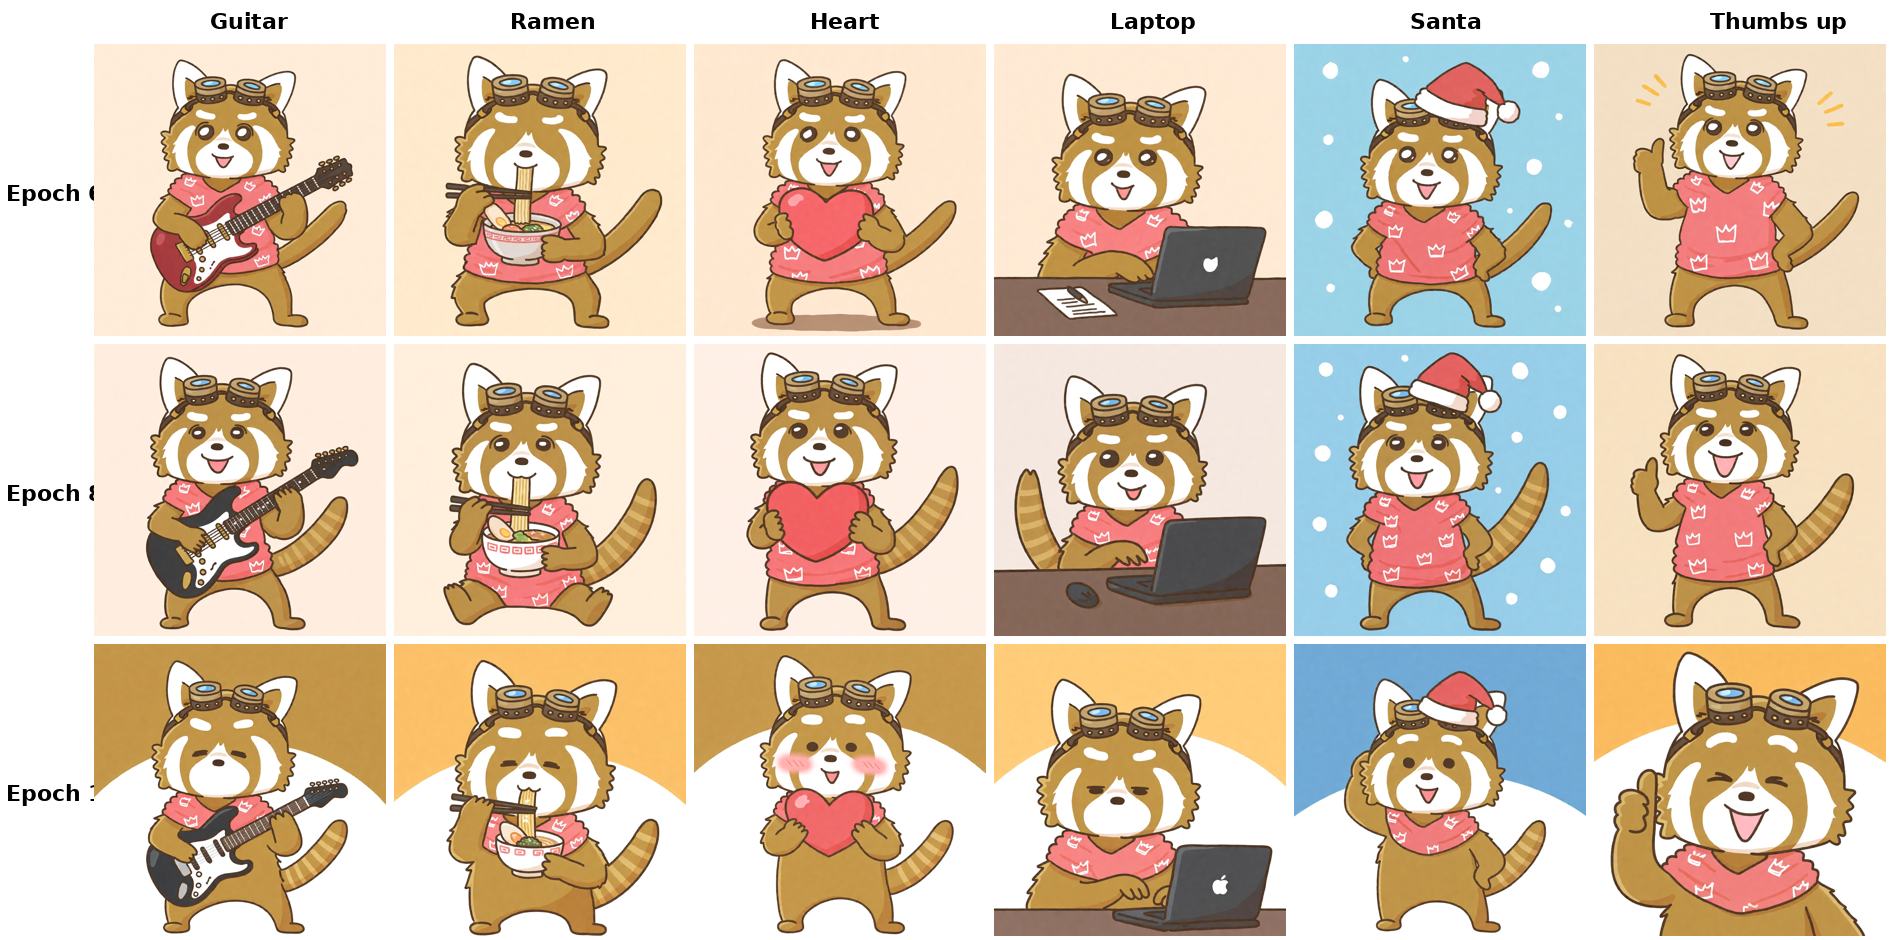
\includegraphics[width=0.92\textwidth]{figures/fig_epoch.png}
\caption{エポックアブレーション（行：エポック6/8/10、列：6ポーズ、同一乱数種）。エポック10は全体造形が最も濃いが、背景が暖色へ偏り、目のキャッチライトが失われる過適合傾向を示す。}
\label{fig:epoch}
\end{figure*}

\subsection{推論時介入による品質制御}
学習後の介入のみでエポック10の造形と細部を両立できるかを検討した。図\ref{fig:eye} に、(A) エポック10・適用強度 $\lambda=1.0$、(B) エポック10・$\lambda=0.8$、(C) エポック10・$\lambda=1.0$＋目の高光点を明示するプロンプト、(D) 参照としてエポック8・$\lambda=1.0$、を比較する。$\lambda$ の低減（B）は過適合の効きを緩めて細部を部分的に回復させ、プロンプト条件付け（C）はエポック10の造形を保ったままキャッチライトを呼び戻した。両者の併用（$\lambda=0.8$＋プロンプト）が、全体造形と高周波細部の最良の折衷を与えた。これは、再学習を要さずとも、適用強度（式\eqref{eq:lora}の $\lambda$）とテキスト条件の二つの推論時自由度により、過適合の副作用を実用的に制御できることを示す。

\begin{figure}[t]\centering
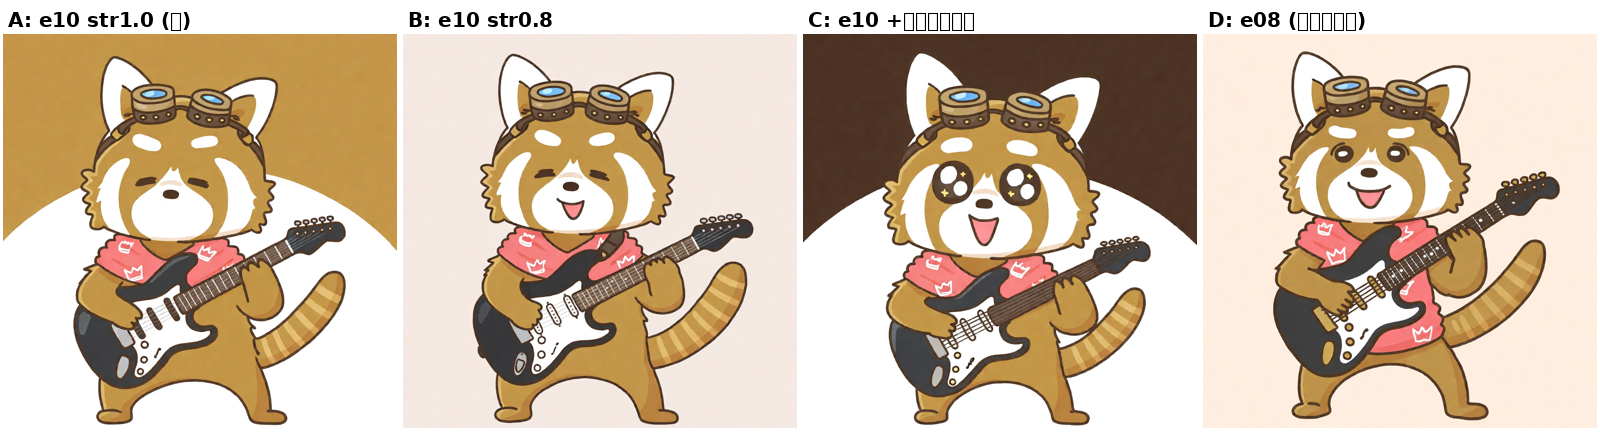
\includegraphics[width=0.96\columnwidth]{figures/fig_eye.png}
\caption{目のキャッチライトの回復。(A) e10, $\lambda{=}1.0$、(B) e10, $\lambda{=}0.8$、(C) e10, $\lambda{=}1.0$＋目の高光点プロンプト、(D) e8（参照）。$\lambda$低減とプロンプト条件付けで高周波細部が回復する。}
\label{fig:eye}
\end{figure}

\section{考察}
\textbf{規模拡大に対する枠組みの頑健性。} 先行研究~\cite{suzuki2026sd15lora} は約10億パラメータの U-Net に対する個人キャラクタ学習を消費者向けGPUで実証した。本研究はこれを約12倍規模の120億パラメータ MMDiT へ拡張しても、同一のGPUで枠組みが成立することを示した。両者の差は学習対象の規模と数値・メモリ戦略にあり、被写体・データ規模・GPUは共通である。すなわち、「個人が所有するキャラクタの追加学習は消費者向けGPU 1台で完結する」という主張は、世代をまたいで頑健であった。

\textbf{過適合の周波数的非対称性。} E3で観察された「高周波の細部が低周波の造形より先に劣化する」現象は、少数データ・キャラクタLoRAにおけるエポック選定の指針を与える。最終エポックが必ずしも最良ではなく、細部の保存を重視するならばより早いエポック、あるいは推論時の適用強度低減が有効である。重要なのは、この劣化が破壊的ではなく、推論時の二自由度（$\lambda$ とテキスト条件）で可逆的に補償できる点である。

\textbf{学習・推論の分業。} RAW で学習し Turbo で推論する構成は、学習の数値的安定性（高精度なRAW）と推論の効率（8ステップ・省メモリなTurbo）を両立させた。蒸留モデルが学習対象として扱いにくい場合に、蒸留前モデルを学習に充てる本構成は一般的な指針となりうる。

\section{限界と今後の課題}
本研究には次の限界がある。第一に、スループットは約23.2\,秒/ステップとSD~1.5の学習に比して大きく、これはブロックスワップに伴う CPU--GPU 間転送が支配的要因である。第二に、ブロックスワップは主記憶を圧迫し、学習中は他のGPU・メモリ常駐サービスの一時停止を要した。第三に、評価は主として定性的であり、同一性の定量指標（埋め込み類似度など）や被験者評価は今後の課題である。第四に、エポックは2刻みでのみ保存しており、過適合が顕在化する厳密な境界の特定には至っていない。第五に、推論側に量子化（GGUF~Q5\_K\_M）を併用しており、量子化が転移品質に与える影響の切り分けは行っていない。

\section{結論}
本研究は、消費者向け単一GPU（RTX~3060、VRAM 12\,GB）上で、約120億パラメータの最新画像生成モデル Krea~2 に対する個人キャラクタの LoRA 微調整が成立することを実証した。FP8 量子化・ブロックスワップ・メモリ断片化対策の三者併用が本規模での学習の必要条件であり、蒸留前 RAW で学習した LoRA は蒸留版 Turbo の推論へ良好に転移した。さらに、エポック数の増加が高周波の細部を先に劣化させる過適合の非対称性を観察し、これが推論時の適用強度とテキスト条件により可逆的に補償可能であることを示した。先行研究の結論——個人キャラクタの追加学習は有料クラウド資源を用いずとも消費者向けGPU 1台で完結する——は、一桁規模の大きい最新世代モデルにおいても引き続き成立する。

\section{主要ハイパーパラメータ}
拡散モデル: Krea~2 RAW（学習）／ Turbo GGUF~Q5\_K\_M（推論）。テキストエンコーダ: Qwen3-VL-4B（bf16）。VAE: Qwen-Image VAE。LoRA: 階数 $r=32$、$\alpha=32$、対象は MMDiT 線形層。最適化: AdamW、学習率 $1\times10^{-4}$、バッチサイズ1、勾配チェックポインティング有効。時刻サンプリング: シフト、$\sigma=2.5$。総ステップ: 1{,}300（10エポック）。省メモリ: FP8スケール量子化＋ブロックスワップ26＋\texttt{expandable\_segments}。解像度: $1024\times1024$。推論: \texttt{er\_sde}／\texttt{simple}／8ステップ／$s=1.0$。採用設定: エポック10、適用強度 $\lambda=0.8$、目の高光点を明示するプロンプトを併用。

\section{再現環境}
GPU: NVIDIA GeForce RTX~3060（VRAM 12\,GB、ドライバ 595.71.05）。主記憶: 30\,GB。PyTorch: 2.6.0+cu124。学習基盤: Musubi Tuner~\cite{musubi2026}（コミット \texttt{30c658c}）。学習時間: 8時間23分（約23.2\,秒/ステップ）。最終損失: 0.0269。

\begin{thebibliography}{9}
\bibitem{suzuki2026sd15lora} M.~Suzuki. 個人制作キャラクターの画像生成LoRAファインチューニング——消費者向けGPUを用いた少数データ条件下での実験的検討——. 技術報告, 2026.
\bibitem{ho2020ddpm} J.~Ho, A.~Jain, and P.~Abbeel. Denoising Diffusion Probabilistic Models. \textit{Advances in Neural Information Processing Systems (NeurIPS)}, 2020.
\bibitem{rombach2022ldm} R.~Rombach, A.~Blattmann, D.~Lorenz, P.~Esser, and B.~Ommer. High-Resolution Image Synthesis with Latent Diffusion Models. \textit{IEEE/CVF Conference on Computer Vision and Pattern Recognition (CVPR)}, 2022.
\bibitem{peebles2023dit} W.~Peebles and S.~Xie. Scalable Diffusion Models with Transformers. \textit{IEEE/CVF International Conference on Computer Vision (ICCV)}, 2023.
\bibitem{esser2024sd3} P.~Esser, S.~Kulal, A.~Blattmann, et al. Scaling Rectified Flow Transformers for High-Resolution Image Synthesis. \textit{International Conference on Machine Learning (ICML)}, 2024.
\bibitem{lipman2023flowmatching} Y.~Lipman, R.~T.~Q. Chen, H.~Ben-Hamu, M.~Nickel, and M.~Le. Flow Matching for Generative Modeling. \textit{International Conference on Learning Representations (ICLR)}, 2023.
\bibitem{hu2022lora} E.~J.~Hu, Y.~Shen, P.~Wallis, Z.~Allen-Zhu, Y.~Li, S.~Wang, L.~Wang, and W.~Chen. LoRA: Low-Rank Adaptation of Large Language Models. \textit{International Conference on Learning Representations (ICLR)}, 2022.
\bibitem{ruiz2023dreambooth} N.~Ruiz, Y.~Li, V.~Jampani, Y.~Pritch, M.~Rubinstein, and K.~Aberman. DreamBooth: Fine Tuning Text-to-Image Diffusion Models for Subject-Driven Generation. \textit{IEEE/CVF Conference on Computer Vision and Pattern Recognition (CVPR)}, 2023.
\bibitem{qwenimage2025} Qwen Team. Qwen-Image Technical Report. 2025.
\bibitem{micikevicius2022fp8} P.~Micikevicius, D.~Stosic, N.~Burgess, et al. FP8 Formats for Deep Learning. arXiv:2209.05433, 2022.
\bibitem{musubi2026} kohya-ss. Musubi Tuner. \url{https://github.com/kohya-ss/musubi-tuner}, 2026.
\end{thebibliography}

\end{document}
